\documentclass[tikz,border=20pt]{standalone}
\usepackage{amsmath, amssymb}
\usetikzlibrary{positioning, shapes.geometric, fit, backgrounds, decorations.pathmorphing}

\newcommand{\Z}{\mathbb{Z}}
\newcommand{\C}{\mathbb{C}}
\newcommand{\F}{\mathbb{F}}
\newcommand{\Spec}{\operatorname{Spec}}

\begin{document}
	
	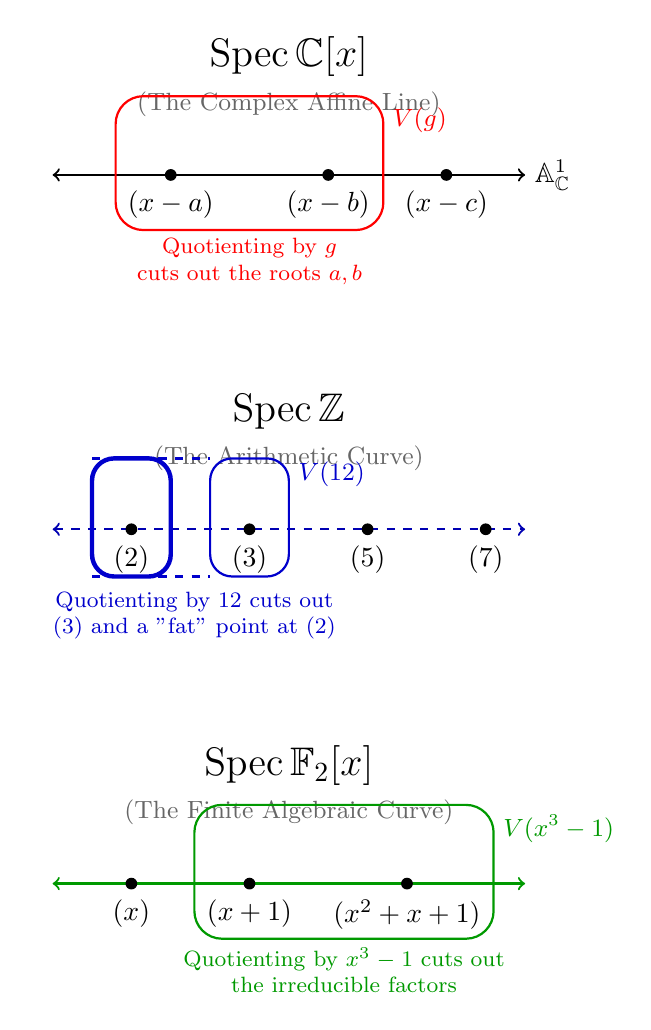
\begin{tikzpicture}[
		point/.style={circle, fill=black, inner sep=1.5pt},
		fatpoint/.style={circle, fill=black, inner sep=2.5pt},
		locus/.style={draw, rounded corners=10pt, dashed, thick, inner sep=8pt},
		node distance=1.5cm
		]
		
		% ==========================================
		% 1. The Complex Line: Spec C[x]
		% ==========================================
		\node[font=\Large\bfseries] at (0, 0) {$\Spec \C[x]$};
		\node[font=\small, text=gray!80!black] at (0, -0.6) {(The Complex Affine Line)};
		
		% The continuous line
		\draw[thick, <->] (-3, -1.5) -- (3, -1.5);
		\node[right] at (3, -1.5) {$\mathbb{A}^1_\C$};
		
		% Points
		\node[point, label=below:{$(x-a)$}] (pa) at (-1.5, -1.5) {};
		\node[point, label=below:{$(x-b)$}] (pb) at (0.5, -1.5) {};
		\node[point, label=below:{$(x-c)$}] (pc) at (2, -1.5) {};
		
		% Vanishing Locus for g(x) = (x-a)(x-b)
		\draw[red, thick, rounded corners=10pt] 
		(-2.2, -2.2) rectangle (1.2, -0.5);
		\node[red, font=\small, right] at (1.2, -0.8) {$V(g)$};
		\node[red, font=\footnotesize, text width=3cm, align=center] at (-0.5, -2.6) 
		{Quotienting by $g$\\cuts out the roots $a, b$};
		
		
		% ==========================================
		% 2. The Arithmetic Line: Spec Z
		% ==========================================
		\begin{scope}[yshift=-4.5cm]
			\node[font=\Large\bfseries] at (0, 0) {$\Spec \Z$};
			\node[font=\small, text=gray!80!black] at (0, -0.6) {(The Arithmetic Curve)};
			
			% The discrete/bumpy line (drawn as a line to show connection)
			\draw[thick, <->, dashed, color=blue!70!black] (-3, -1.5) -- (3, -1.5);
			
			% Points (Prime numbers)
			\node[point, label=below:{$(2)$}] (p2) at (-2, -1.5) {};
			\node[point, label=below:{$(3)$}] (p3) at (-0.5, -1.5) {};
			\node[point, label=below:{$(5)$}] (p5) at (1, -1.5) {};
			\node[point, label=below:{$(7)$}] (p7) at (2.5, -1.5) {};
			
			% Vanishing Locus for (12) = (2^2 * 3)
			% Make the circle around 2 thicker to represent multiplicity (fat point)
			\draw[blue!80!black, ultra thick, rounded corners=8pt] (-2.5, -2.1) rectangle (-1.5, -0.6);
			\draw[blue!80!black, thick, rounded corners=8pt] (-1, -2.1) rectangle (0, -0.6);
			\draw[blue!80!black, thick, dashed] (-2.5, -2.1) -- (-1, -2.1) (-2.5, -0.6) -- (-1, -0.6);
			
			\node[blue!80!black, font=\small, right] at (0, -0.8) {$V(12)$};
			\node[blue!80!black, font=\footnotesize, text width=4cm, align=center] at (-1.2, -2.6) 
			{Quotienting by $12$ cuts out\\$(3)$ and a "fat" point at $(2)$};
		\end{scope}
		
		
		% ==========================================
		% 3. The Finite Affine Line: Spec F2[x]
		% ==========================================
		\begin{scope}[yshift=-9cm]
			\node[font=\Large\bfseries] at (0, 0) {$\Spec \F_2[x]$};
			\node[font=\small, text=gray!80!black] at (0, -0.6) {(The Finite Algebraic Curve)};
			
			% The line
			\draw[thick, <->, color=green!60!black] (-3, -1.5) -- (3, -1.5);
			
			% Points (Irreducible polynomials over F2)
			\node[point, label=below:{$(x)$}] (px) at (-2, -1.5) {};
			\node[point, label=below:{$(x+1)$}] (px1) at (-0.5, -1.5) {};
			\node[point, label=below:{$(x^2+x+1)$}] (px2) at (1.5, -1.5) {};
			
			% Vanishing Locus for x^3-1 = (x+1)(x^2+x+1) over F2
			\draw[green!60!black, thick, rounded corners=10pt] 
			(-1.2, -2.2) rectangle (2.6, -0.5);
			\node[green!60!black, font=\small, right] at (2.6, -0.8) {$V(x^3-1)$};
			\node[green!60!black, font=\footnotesize, text width=4.5cm, align=center] at (0.7, -2.6) 
			{Quotienting by $x^3-1$ cuts out\\the irreducible factors};
		\end{scope}
		
	\end{tikzpicture}
	
\end{document}